\documentclass[12pt,a4paper,final]{report}
\usepackage[utf8]{inputenc}
\usepackage[english]{babel}

% Package fo use of url
\usepackage{url}

% Packages for math symbols
\usepackage{amsmath}
\usepackage{amsfonts}
\usepackage{amssymb}
\usepackage[amssymb]{SIunits}

% Packages for images
\usepackage[final,pdftex]{graphicx}
\usepackage{float}

% Package for header
\usepackage{fancyhdr}
\setlength{\headheight}{15.2pt}
\renewcommand{\headrulewidth}{0pt}
\renewcommand{\footrulewidth}{0pt}

% Package for dividing sections
\usepackage{parskip}

\numberwithin{equation}{section}
\numberwithin{table}{section}
\numberwithin{figure}{section}

\renewcommand*\thesection{\arabic{section}} % fix to hide chapter number

\author{Hans-Kristian Bruvold\\Tom Eivind Glover\\Torkel Berli}
\title{Exercise 2 report}
\date{2013-03-15}

%\fancyhf{}

\renewcommand{\thispagestyle}[1]{} % do nothing


\begin{document}

\begin{titlepage} % TITLE ###################################

\pagestyle{fancy}
\chead{TDT4258 - Energy Efficient Computer Design}
\rhead{}
\cfoot{}
\begin{center}

\bigskip
\textbf{\LARGE REPORT}\\
\vspace{1.5cm}
\textnormal{\LARGE Exercise 2}\\
\vspace{1cm}
\textbf{\LARGE Sound using ABDAC}\\

\vspace{3cm}
by
\\
\vspace{0.5cm}
Hans-Kristian Bruvold\\
Tom Eivind Glover\\
Torkel Berli\\


\vspace{9cm}
Date: 2013-03-15

\end{center}

\end{titlepage} % END TITLE ###############################

\pagestyle{fancy}
\chead{}
\lhead{}


\section*{Abstract}
\label{sec:abstract} % a label to refer to

In this exercise we will produce sound from an Atmel STK1000 development board. Doing so will require knowledge about generating interrupts from a clock in the power manager of the microcontroller to have a flow of sample data sent to the speakers through a ABDAC, Audio Bitstream Digital to Analogue Converter. The program is to be written in C, and then compiled using the GNU-toolchain and libraries for the microcontroller and its processor.

\newpage

\tableofcontents

\newpage

\clearpage
\pagenumbering{arabic}

\cfoot{\thepage}

\section{Introduction}
\label{sec:introduction}
This report will explain how we got sound playing from the Atmel STK1000 development board. The report will cover the theory behind sound, what tools we will use on the Atmel STK1000 development board to generate sound, how we approach the problem and the result with conclusion.

Sound is compression and decompression of air in motion. We usually talk about sound as waves with amplitude and frequency. The amplitude is how much the air is compressed/decompressed from the default pressure. And the frequency is how often the pressure switches from compressed to decompressed state. A speaker will generate the sound. So our task in this exercise is to send data to the speaker in order to get the sound we want. 

\newpage

\section{Methodology}
\label{sec:methodology}

\subsection{Atmel STK1000 development board}
\label{sec:stk1000}
As mentioned earlier, we will be using the Atmel STK1000 development board. 


\begin{figure}[H]
\centering
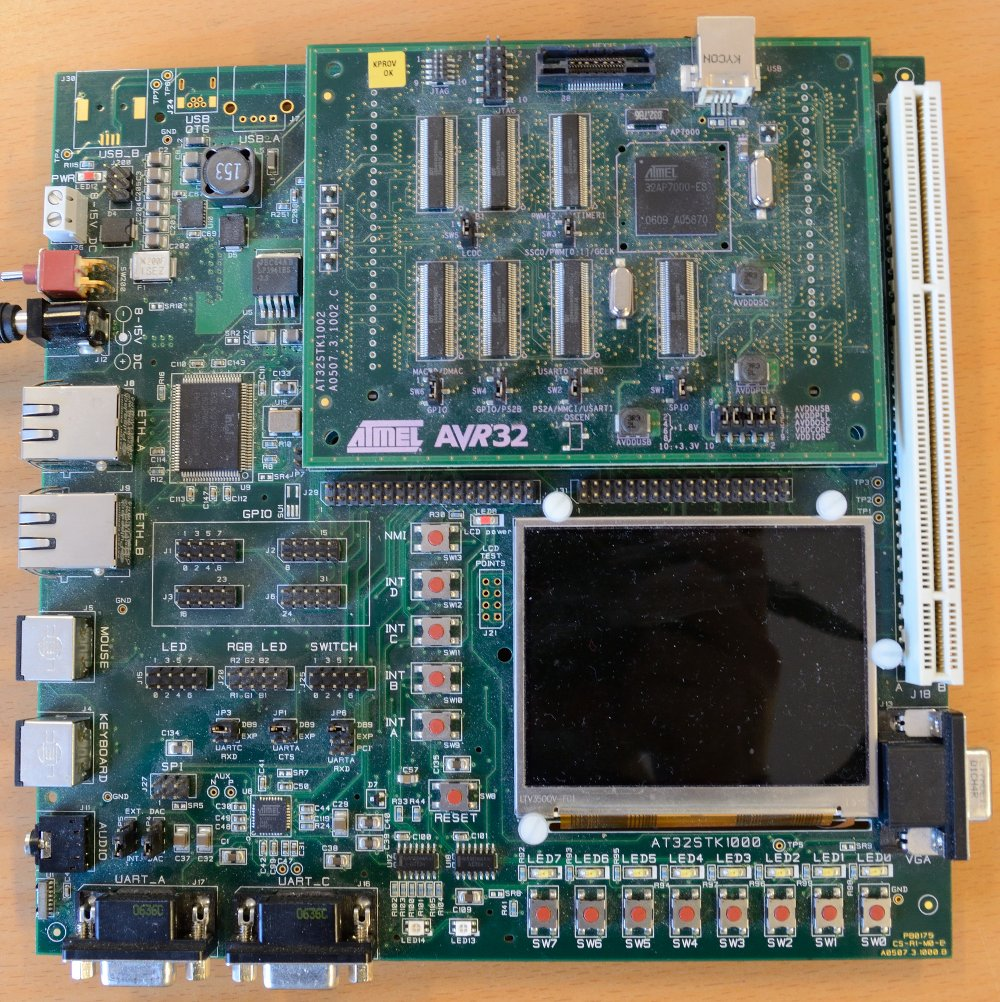
\includegraphics[scale=1.5]{stk1000photo}
\caption{Atmel STK1000 development board}
\label{fig:stk1000}
\end{figure}

The features relevant with this exercise are the GPIO - General Purpose Input Output, PIO controller - Parallel Input Output Controller, interrupt controller, power manager and ABDAC - Audio Bitstream Digital to Analog Converter.

The development board can be programmed using a JTAG, Joint Test Action Group. The JTAG can be used for both debugging and programming by using Atmel's own binaries for the board. 

\subsection{PIO Controller}
\label{sec:pio}

\begin{figure}[H]
\centering
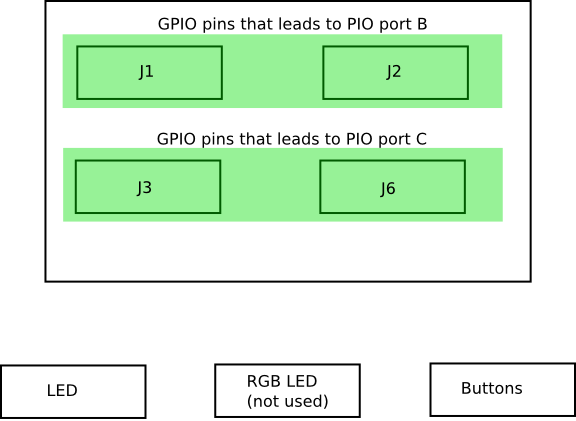
\includegraphics[scale=0.5]{gpio}
\caption{GPIO - General Purpose Input Output}
\label{fig:gpio}
\end{figure}

The GPIO works as a hardware switch using ribbon cable to connect LEDs and buttons to the PIO Controller. The PIO Controller has a set of ports connected to different sources. Some pins on port B and C are connected to the GPIO. As seen in Figure \ref{fig:gpio}, the GPIO features connection to LEDs and buttons.

As said, the PIO controller is also connected to different sources. Not all pins of port B and C are connected to the GPIO, some pins are connected to the Power Manager. This means that the Power Manager is connected through the PIO Controller and can be as input on various components, including the ABDAC.

\begin{table}[H]
\centering
\begin{tabular}{|l|l|}
\hline
Name & Register\\
\hline
PER & PIO Enable Register\\
PDR & PIO Disable Register\\
OER & Output Enable Register\\
PUER & Pull-Up Enable Register\\
IER & Interrupt Enable Register\\
SODR & Set Output Data Register\\
CODR & Clear Output Data Register\\
PDSR & Pin Data Status Register\\
ASR & Peripheral A Select Register\\
\hline
\end{tabular}
\caption{Some of the control registers for the PIO Controller, for full list see page 262-263 in AT32AP7000 data sheet\cite{at32ap7000}}
\label{tab:pioregisters}
\end{table}

The pins on a PIO port has to be correctly configured in order to function as it is supposed to. So every pins have a set of settings that can be configured through virtual memory addresses. Some of the registers are shown in Table \ref{tab:pioregisters}.

The correct configuration for LEDs is first to enable the correct pins by setting bit '1' to the PER register. All the pins on the PIO are configured by default to be used as input, so this has to be changed for the LED pins. Writing '1' to the pins used for LEDs to the OER register. Now the LEDs are configured and can be turned on by writing '1' to the bits in the SODR register and turned off by writing '1' to the bits in the CODR register.

In order to configure buttons, the correct pins has to be enabled in the same way as for LEDs. Then They have to be set to use pull-up resistors, which is done by writing '1' to the bits in the PUDR register. Now, if the PIO controller is to fire an interrupt when a change has happened to the buttons, the bits in the IER register has to be enabled. The PDSR register can be read to get the current button state, '1' means that a button is not pressed.

The setup for using the Power Manager through PI and connect them to the ABDAC, the pin 20 and 21 has to be configured. First the pins has to be disabled by setting the bits in PDR register to '1', this is done so that the PIO is not in control of the pins. Then the pins has to be connected to Peripheral A, which is the ABDAC. This is done by writing '1' to the bits n the ASR register.

\subsection{Power Manager}
\label{sec:powermanager}

The Power Manager is what will be used to control oscillators and generate clocks. It has two kinds of oscillators, one is running at 12 MHz, while the other is running at 20 MHz. The Power Manager has 8 generic clocks, number 6 is allocated for the DAC. 

\begin{table}[H]
\centering
\begin{tabular}{|l|l|}
\hline
Name & Function\\
\hline
DIV & Division factor\\
DIVEN & Use division\\
CEN & Clock enable\\
PLLSEL & Select PLL as clock, else oscillator\\
OSCSEL & Select PLL/oscillator clock source\\
\hline
\end{tabular}
\caption{Config bits for generic clocks in Power Manager, see page 118 AT32AP7000 data sheet\cite{at32ap7000}}
\label{tab:genericclock}
\end{table}

For configuring the clock to be used as ABDAC controller, the bits in Table \ref{tab:genericclock} has to be correctly set. The CEN bit is easy, it has to be '1' in order for the clock to be running. The PLL is a clock that takes a generic clock as source clock and ether divide or multiply the clock frequency. For ABDAC, this is not nececary, as the generic clock gives a good frequency for the ABDAC. So setting the PLLSEL to '0', also means that the DIVEN also have to be '0'. It is best to use the 12 MHz generic clock for the ABDAC as it will make the ABDAC sample rate 48 kHz, see Section \ref{sec:abdac}. The oscillator 1 generates 12 MHz, so the OSCSEL should be set to '1'.


\subsection{ABDAC}
\label{sec:abdac}

The ABDAC, or Audio Bitstream Digital to Analogue Converter, is the component that takes digital data, and converts it to analogue signal. It does this by repeatedly asking for new sample data. The sample data is basically an 16-bit signed integer. The sample data is converted to a voltage and put on the audio output jack. So if the stream of sample data represents a wave of some kind (like sinus, sawtooth, square, etc.), the speaker will produce compressions and decompressions of air, as talked about in the introduction, which basically is sound. 

Just as the PIO controller, the ABDAC has a set of virtual memory addresses which is used for configuring the ABDAC. The relevant options for using ABDAC with the generick clock, is by using interrupts. Interrupts can be enabled through the IER register of the ABDAC. By setting the TX\_READY bit to '1', the ABDAC will generate an interrupt when it is ready to receive a new sample data. Another bit that has to be enabled is the EN bit in the Control Register (CR), this will enable the use of the ABDAC.


\subsection{Interrupts}
\label{sec:interrupts}

In order to use interrupts, the CPU has to be configured to respond to interrupts and the Interrupt Controller has to be configured to receive interrupt requests and transmit interrupts. 

The CPU's configuration is to set the system register EVBA (Exception Vector Base Address). It is used to store the base address of the interrupt routine in the program code, and must be configured whenever interrupts are implemented.

The interrupt controller has 64 groups of interrupt signals. Each group supports 32 different interrupt sources. When the interrupt controller receives an interrupt request signal from a source in one of its 64 groups, it initiates an interrupt call specific to that group to the microprocessor. This interrupt call consists of a priority level and an autovector. The autovector is an address offset from the base address for interrupts (EVBA) in the program code. By using the autovector, the program code can have a separate interrupt routine for each interrupt group in the interrupt controller. 

Setting the EVBA using C, is as easy as running a function from a interrupt library. And when setting the interrupt controller to listen to different interrupts, it's another function to run. This function needs the group number and the interrupt source number. These numbers can be calculated from the IRQ address which can be fetched from the controller library. The group number is IRQ divided by 32, and the interrupt source number is IRQ modulo 32.

\newpage

\section{Description}
\label{sec:description}

\subsection{Progress}
\label{sec:progress}

We started this exercise by creating a Makefile. We made it as general as possible. That way we needed only to change one line when adding more files to the project. 

After we had a working Makefile we started with the program. We started of with just simply turning on LEDs when a button was pressed. We did this using interrupts. And that was pretty straight forward. 

When the LEDs and buttons worked, we tried giving the ABDAC random data using the rand() from stdlib.h library. When we got the noise we expected, we could continue.

The next step was a huge step. By now, we added other files. Actually all the files in the final program was done in this step. The only errors that appeared under compiling was typos. There were some smaller bugs when trying to run it on the STK1000. These bugs weren't hard to find, so we didn't take the time to use any debugging tools. 

\subsection{Code description}
\label{sec:codedescription}


\begin{figure}[H]
\centering
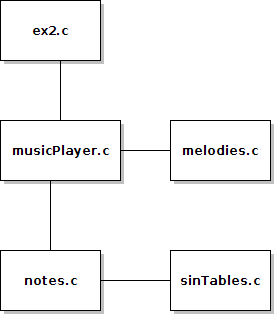
\includegraphics[scale=0.5]{fileStructure}
\caption{Overview of the file structure}
\label{fig:filestructure}
\end{figure}

Figure \ref{fig:filestructure} shows an overview on the file structure. The ex2.c is the main file. It contains the initialisation code for buttons, LEDs, interrupts, Power Manager and ABDAC. It also contains interrupt routine for buttons and for the ABDAC.

The musicPlayer.c has the task of having control of what melody is playing, and the position of the melody. It has a function getNextSample() which returns the next sample data for the ABDAC. That way, the only thing that needs to be in the interruct routine in ex2.c is getNextSample(). ex2.c don't have to handle what the next note for the melody is.

The melodies.c is just a simple file that acts as a data storage. It does not have any functions, only variables. All the melodies are stored in this file. There are also variables available to adjust the speed of each melody.

The notes.c is the file handling the sinus tables. It has a function to get a short int in a specified position in for one note. It also handles the calculation between different octaves.

The sinTables.c is the file that stores all the sinus tables for the different notes. That is the only purpose of this file.


\subsection{Sound representation}
\label{sec:soundrepresentation}

The solution we chose to this exercise was to use one sinus table for each note, and then skip some entries or play some more than once. The sinus tables are just array of short int which was extracted from a sinus function. We used a python script to generate the tables. There is one table per note, as said. So when we wanted to go one octave up, we could just play every other entry of the array. And when we wanted to go one octave down, we used each entry twice. 

The melodies was stored as char arrays. Each note consisted of 3 chars. The first was the note itself. The second char was the octave. And the Third char war divisor for how long the note lasted. So a half note of C4, would be "c42".

The melodies we have created so far is intended to be intro, win and lose sounds. Some of the other are for testing.


\newpage

\section{Results}
\label{sec:results}

We actually didn't do that much testing in this exercise. The first basic things like the LEDs and buttons, worked right away. Also when sending rand() data to the ABDAC, it worked once we tried it. So the only testing we did on the first steps, was testing that things worked by watching the result when running the program on the board. We didn't have any reasons to believe that there was something else wrong in the code. So no further testing was necessary at this point.

When checking the final code, we compiled it and checked if we got the expected result when running the program. The sound from the final result does suffer from a bit noise between notes. The noise between the notes is like when you have your headphones on and snap out the audio jack. Also the notes did not sound as clear as we expected.

The melody data could also be fitted better to suit the way the application handles the melodies. You can easily hear that there are different melodies when pressing the different buttons, but they're not that easy to identify what they are melodies from. 

\newpage

\section{Discussion}
\label{sec:discussion}

\subsection{DMA vs interrupts}
\label{sec:dmainterrupt}
We discussed early the possibility to use DMA to send the sound to the ABDAC but decided not to after conferring with the und. ass. who advised against it as this would require substantially more work then the project was intended to. If we had done it though, the energy cost from the system would go down compared to the alternative when the music was playing. By using DMA you could be able to put the CPU to sleep while one song is playing. 

\subsection{Alternative waves}
\label{sec:alternativewaves}
The tables we generated was only made by the sinus sinus function. More experimenting with other types of functions to generate other waves is one thing that could give better sound experience. 

\subsection{Alternative sample source}
\label{sec:alternativesamplesource}
The cause of the unclear sound and the noise in between notes, are most likely caused by the use of sample tables. The change from one note to silence or another note is too sudden. When switching from sample data which is on the top of the wave to sample data at zero, will make a spiky noise. Using something else than sample tables would probably solve most of this issue, depending on the alternate solution of course.

\subsection{Alternative sound representation}
\label{sec:alternativesoundrepresentation}
We chose the represent our sound not entirely dissimilar to how MIDI files represent sound as they also map a value to a specific sound, but they would represent C4 just as a number lets say 60. The MIDI files would also have the opportunity to map the numbers to different sounds which we did not do. This could possibly be possible to execute, but would require more experience and deeper understanding on how to generate sound.

\newpage

\section{Conclusion}
\label{sec:conclusion}
We should have devoted more time to this exercise, but sadly we were all very busy with other elements of our study at the same time, so we did not put aside enough time to this project. Nevertheless, we learned a lot from this assignment ranging from C programming to ABDAC management to the relation between notes and octaves in sound. The result does not quite feel final and are subject to improvement prior to its use in exercise 3. 


\bibliographystyle{plain}
\bibliography{bibliography}

\end{document}
